%%%%%%%%%%%%%%%%%%%%%%%%%%%%%%%%%%%%%%%%%
% Stylish Article
% LaTeX Template
% Version 2.2 (2020-10-22)
%
% This template has been downloaded from:
% http://www.LaTeXTemplates.com
%
% Original author:
% Mathias Legrand (legrand.mathias@gmail.com) 
% With extensive modifications by:
% Vel (vel@latextemplates.com)
%
% License:
% CC BY-NC-SA 3.0 (http://creativecommons.org/licenses/by-nc-sa/3.0/)
%
%%%%%%%%%%%%%%%%%%%%%%%%%%%%%%%%%%%%%%%%%

% SNIPPET UTILI %


%----------------------------------------------------------------------------------------
%	PACKAGES AND OTHER DOCUMENT CONFIGURATIONS
%----------------------------------------------------------------------------------------

\documentclass[fleqn,10pt]{SelfArx} % Document font size and equations flushed left

%\usepackage[english]{babel} % Specify a different language here - english by default
\usepackage[italian]{babel} % Specify a different language here - english by default

\usepackage{lipsum} % Required to insert dummy text. To be removed otherwise

%----------------------------------------------------------------------------------------
%	COLUMNS
%----------------------------------------------------------------------------------------

\setlength{\columnsep}{0.55cm} % Distance between the two columns of text
\setlength{\fboxrule}{0.75pt} % Width of the border around the abstract

%----------------------------------------------------------------------------------------
%	COLORS
%----------------------------------------------------------------------------------------

\definecolor{color1}{RGB}{0,0,90} % Color of the article title and sections
\definecolor{color2}{RGB}{0,20,20} % Color of the boxes behind the abstract and headings

%----------------------------------------------------------------------------------------
%	HYPERLINKS
%----------------------------------------------------------------------------------------

\usepackage{hyperref} % Required for hyperlinks

\hypersetup{
	hidelinks,
	colorlinks,
	breaklinks=true,
	urlcolor=color2,
	citecolor=color1,
	linkcolor=color1,
	bookmarksopen=false,
	pdftitle={Title},
	pdfauthor={Author},
}

%----------------------------------------------------------------------------------------
%	ARTICLE INFORMATION
%----------------------------------------------------------------------------------------

\JournalInfo{Programmazione per l'IoT - Laurea Magistrale in Informatica Applicata - DiSPeA - Università degli Studi di Urbino Carlo Bo} % Journal information
\Archive{Data di pubblicazione xx/xx/xxxx - DOI: xxxx/xxxxxxx} % Informazioni che verranno inserite dal Docente in fase di pubblicazione

\PaperTitle{4.0 Gym Prototype} % Article title

\Authors{Luca Cinti\textsuperscript{1}*, Emanuele Lattanzi\textsuperscript{2}} % Il docente Emanuele Lattanzi figura come autore
% al fine di poter gestire la procedura di submission sul repository pubblico (nell'affiliazione viene chiarito il ruolo)
\affiliation{\textsuperscript{1}\textit{Laurea Magistrale in Informatica Applicata, Università degli Studi di Urbino Carlo Bo, Urbino, Italia}} % Author affiliation
\affiliation{\textsuperscript{2}\textit{Docente di Programmazione per l'Internet of Things, Università degli Studi di Urbino Carlo Bo, Urbino, Italia}} % Author affiliation
\affiliation{*\textbf{Corresponding author}: l.cinti@campus.uniurb.it} % Corresponding author

\Keywords{IOT --- Arduino --- ESP32 --- MQTT --- Gym Metrics} % Keywords - if you don't want any simply remove all the text between the curly brackets
\newcommand{\keywordname}{Keywords} % Defines the keywords heading name

%----------------------------------------------------------------------------------------
%	ABSTRACT
%----------------------------------------------------------------------------------------

\Abstract{
	In questo elaborato abbiamo cercato di predisporre un'architettura per la raccolta dei dati
	in una piccola home gym, innanzitutto per verificare la fattibilità nel reperimento di alcune misurazioni, 
	per poi passare all'analisi dei dati raccolti, con l'obiettivo di estrapolare delle metriche significative 
	sia ai fini dell'allenamento, che dello studio delle caratteristiche termiche dell'ambiente.
}

%----------------------------------------------------------------------------------------

\begin{document}

\maketitle % Output the title and abstract box

%\tableofcontents % Output the contents section

\thispagestyle{empty} % Removes page numbering from the first page

%----------------------------------------------------------------------------------------
%	ARTICLE CONTENTS
%----------------------------------------------------------------------------------------

\section*{Introduzione} % The \section*{} command stops section numbering
%\lipsum[1-3] % Dummy text
% and some mathematics $\cos\pi=-1$ and $\alpha$ in the text\footnote{And some mathematics $\cos\pi=-1$ and $\alpha$ in the text.}
%Questa è una citazione al libro di testo~\cite{milenkovic2020internet}.

% \begin{enumerate}[noitemsep] % [noitemsep] removes whitespace between the items for a compact look
% 	\item First item in a list
% 	\item Second item in a list
% 	\item Third item in a list
% \end{enumerate}

% \begin{equation}
% 	\cos^3 \theta =\frac{1}{4}\cos\theta+\frac{3}{4}\cos 3\theta
% 	\label{eq:refname2}
% \end{equation}

% \subsection{Subsection}

% \paragraph{Paragraph} \lipsum[7] % Dummy text
% \paragraph{Paragraph} \lipsum[8] % Dummy text

% \subsection{Subsection}

% \lipsum[9] % Dummy text

% Reference to Figure \ref{fig:results}.

% \begin{figure}[ht]\centering
% 	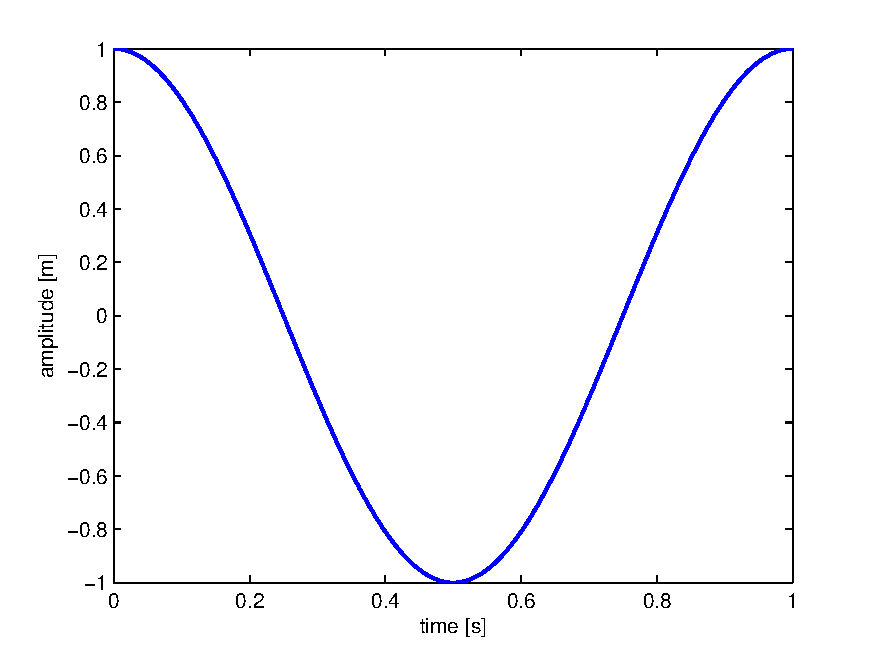
\includegraphics[width=\linewidth]{results}
% 	\caption{In-text Picture}
% 	\label{fig:results}
% \end{figure}

L'obiettivo preliminare di questo elaborato, era verificare la fattibilità dell'allestimento di un sistema di 
raccolta dati in una piccola home gym, costruendo l'infrastruttura per far comunicare, 
attraverso diversi protocolli, una rete di sensori.\\

Tra le più disparate metriche di possibile interesse ai fini dello studio di una palestra, 
sono state scelte due categorie di dati: da un lato i quelli relativi all'ambiente di allenamento, 
dall'altro i dati sull'esecuzione degli esercizi.

Per il progetto corrente, sono state dunque prese in analisi le metriche seguenti:

\begin{itemize}[noitemsep] % [noitemsep] removes whitespace between the items for a compact look
	\item temperatura e umidità della stanza, prima durante e dopo l'allenamento
	\item variazione di CO2 e TVOC (Total Volatile Organic Compounds)
	\item accelerazione del bilanciere durante l'esecuzione di un esercizio campione
\end{itemize}

\section{Descrizione dell'ambiente}

Funzionale alla comprensione di questo elaborato, è la descrizione dell'ambiente in cui è stata allestita 
la palestra: si tratta di una stanza appartenente ad un vecchio immobile disabitato, appositamente 
ristrutturata, le cui misure sono 5.05 x 4.95 metri, per un'altezza di 3.86 metri. \\

L'ambiente presenta una finestra, una porta finestra e un'arcata di ingresso sulla quale sono state applicate 
due tende, fissate con velcro ai lati del muro, come isolante dal resto del locale, in quanto non 
sono presenti sistemi di riscaldamento centralizzato. Possiamo vederne una panoramica nell'immagine che segue 
(Figura 1). \\

\begin{figure*}[ht]\centering % Using \begin{figure*} makes the figure take up the entire width of the page
	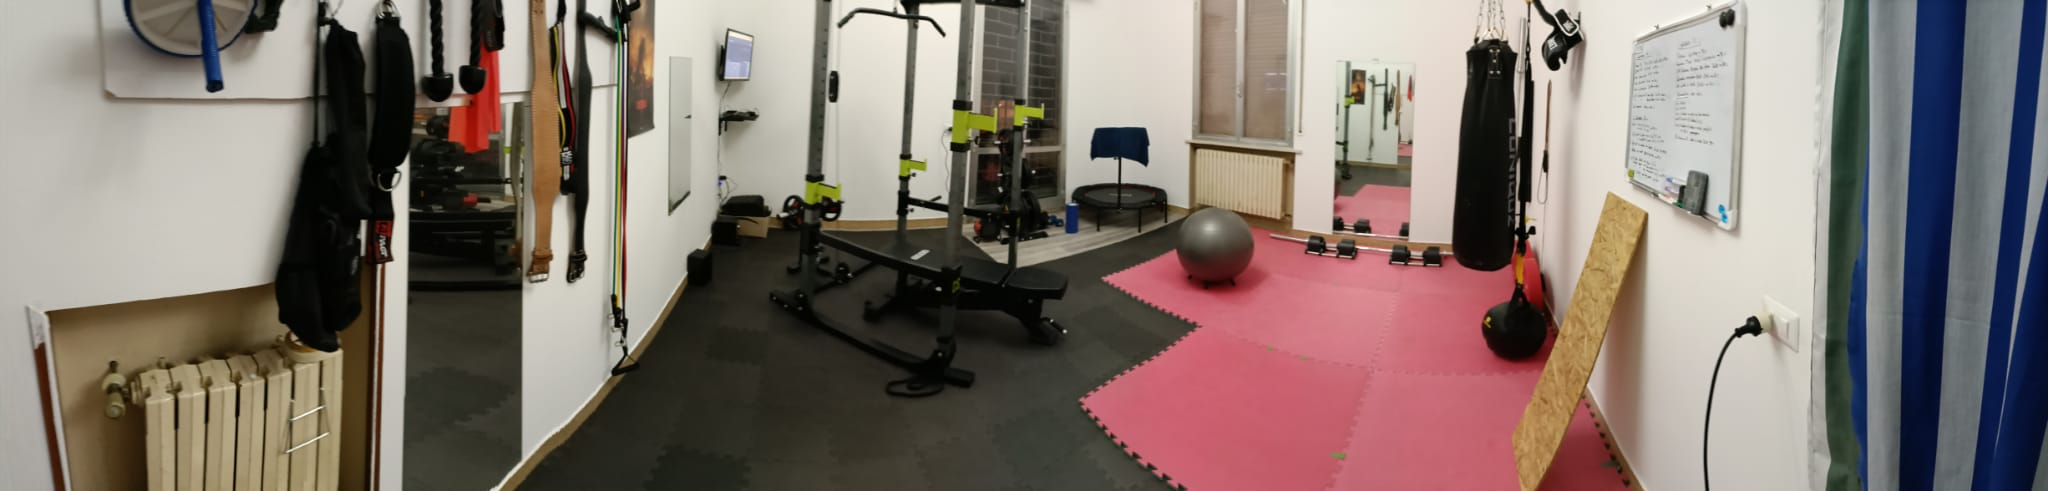
\includegraphics[width=\linewidth]{panoramica_palestra}
	\caption{Visione panoramica dell'ambiente}
	\label{fig:view}
\end{figure*}

Il primo punto di analisi è dunque diretta conseguenza di quanto appena detto: analizzare le performance 
termiche dell'ambiente, per trovare il miglior metodo di riscaldamento durante i mesi invernali.\\
Collegato a questo vi è il secondo punto in analisi: riscaldando un ambiente di circa 96 metri cubici, quanto 
più possibile isolato dal resto del locale, abbiamo ritenuto importante monitorare la qualità dell'aria 
durante l'allenamento.

\section{Scelta della terza metrica}
Come abbiamo visto in precedenza, come terzo oggetto di studio è stata scelta l'accelerazione del bilanciere 
durante l'esecuzione di un esercizio campione.
L'esercizio preso in oggetto è la distensione su panca piana, di cui possiamo vedere uno schema in Figura 2, 
ed è stato scelto in quanto ci garantiva il maggior grado di controllo sull'esecuzione, essendo uno degli 
esercizi base di ogni allenamento. \\
Risultava dunque un ottimo banco di prova sulla fattibilità si questo studio, visto che, data la popolarità 
dell'esercizio, ci consentiva

\begin{figure}[ht]\centering
	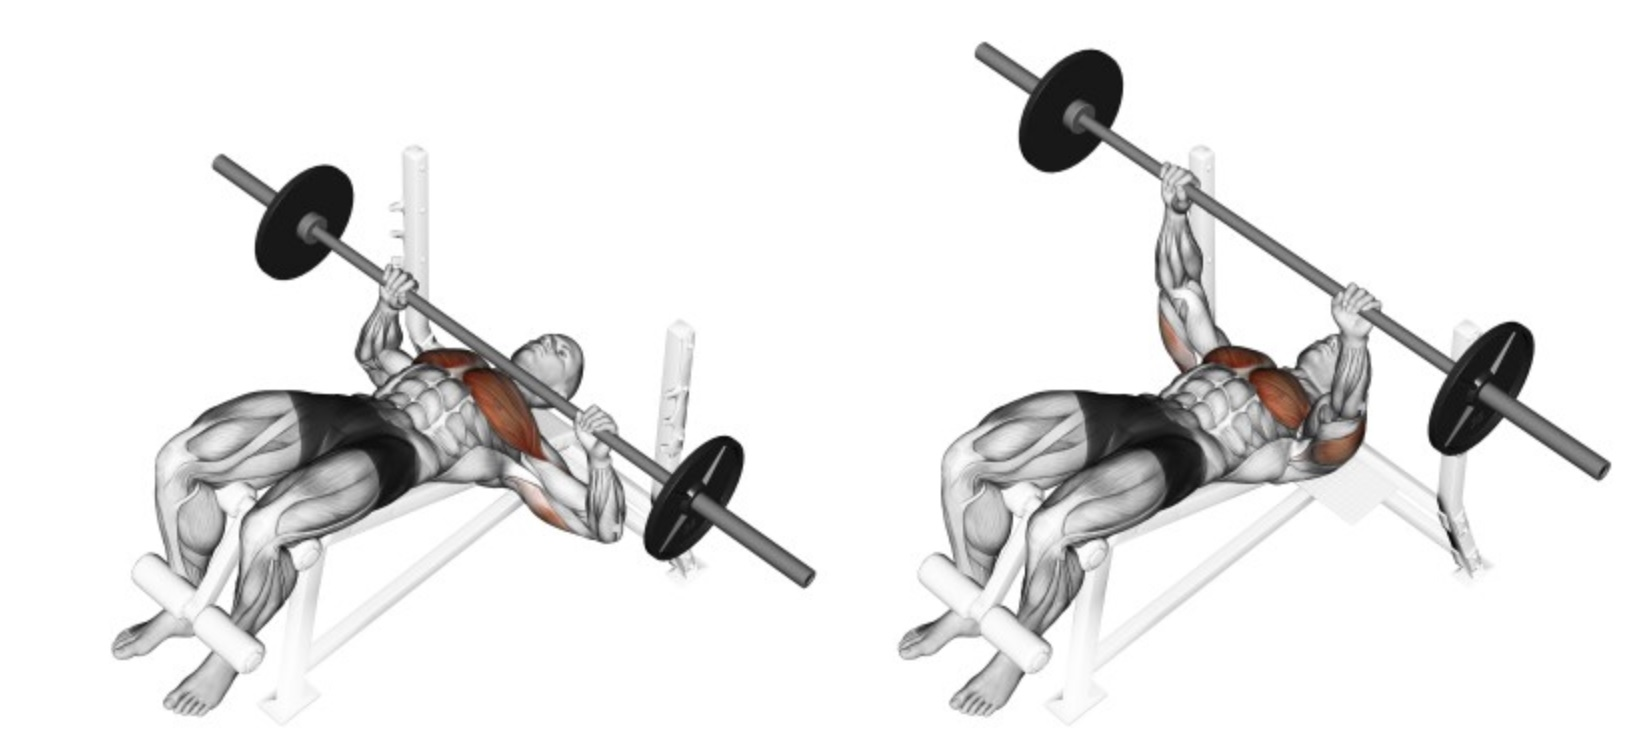
\includegraphics[width=\linewidth]{panca_piana}
	\caption{distensioni su panca piana}
	\label{fig:panca_piana}
\end{figure}

%------------------------------------------------

\section{Risultati}

\lipsum[10] % Dummy text

\subsection{Subsection}

\lipsum[11] % Dummy text

\begin{table}[hbt]
	\caption{Table of Grades}
	\centering
	\begin{tabular}{llr}
		\toprule
		\multicolumn{2}{c}{Name} \\
		\cmidrule(r){1-2}
		First name & Last Name & Grade \\
		\midrule
		John & Doe & $7.5$ \\
		Richard & Miles & $2$ \\
		\bottomrule
	\end{tabular}
	\label{tab:label}
\end{table}

\subsubsection{Subsubsection}

\lipsum[12] % Dummy text

\begin{description}
	\item[Word] Definition
	\item[Concept] Explanation
	\item[Idea] Text
\end{description}

\subsubsection{Subsubsection}

\lipsum[13] % Dummy text



\subsubsection{Subsubsection}

\lipsum[14] % Dummy text

\section{Conclusioni}

\lipsum[15-23] % Dummy text

%----------------------------------------------------------------------------------------
%	REFERENCE LIST
%----------------------------------------------------------------------------------------

\phantomsection
\bibliographystyle{unsrt}
\bibliography{sample.bib}

%----------------------------------------------------------------------------------------

\end{document}
